\documentclass{report}
\usepackage{amsmath}
\usepackage{amssymb}
\usepackage{pgfplots}
\usepackage{siunitx}
\usepackage{algorithm}
\usepackage[noend]{algpseudocode}
\usepackage{graphicx}
\usepackage[export]{adjustbox}
\usepackage{breqn}
\graphicspath{ {./} }
\renewcommand{\figurename}{Figura}
\renewcommand{\contentsname}{Indice}
\renewcommand{\chaptername}{Capitolo}
 
\begin{document}

 \title{Metodi Matematici per il Machine Learning}
\author{Marcello Cuoghi}

\maketitle

\newpage
\begin{abstract}
Piccolo riassunto del corso Metodi Matematici per il Machine Learning interno al corso di laurea magistrale in Ingegneria Informatica presso il dipartimento di Ingegneria Enzo Ferrari, UNIMORE.
\end{abstract}
\newpage

\tableofcontents{}
 
\chapter{Metodo del Gradiente}

\section{Introduzione}
Nel mondo del Machine Learning, si sfrutta il metodo del gradiente per arrivare ad una soluzione del problema di apprendimento che viene espresso in termini di minimizzazione di un funzionale $f: R^n \to R$:

\begin{equation}
    \label{min_funz}
    \min_{x \in R^n} = f(x)
\end{equation}

Questo metodo cerca di sfruttare le informazioni del primo ordine per trovare, con dei piccoli accorgimenti per velocizzarne la convergenza, la soluzione ottima del problema di minimo. Anche se le condizioni del primo ordine spesso non permettono, oltre ad una veloce convergenza, anche una precisione elevata, quest'ultima spesso è irrilevante perché nel caso del Machine Learning una volta addestrato il modello si procede alla nuova classificazione di punti sfruttando operatori quali il segno, e tale operatore risulta insensibile ad una elevata precisione.\\
Nel caso di ricerca del minimo di un funzionale, si deve stabilire se tale minimo esiste e, nel caso, se è globale o locale. Per questo si cerca di utilizzare dove possibile funzionali convessi, che mi garantiscono quindi l'esistenza di un minimo globale e nessun minimo locale. Spesso però questo non è possibile, e quindi si devono eseguire più prove fino al raggiungimento di una soluzione accettabile per il nostro problema. Non è detto che sia sempre possibile arrivare al globale, e spesso non è neanche necessario poiché già un minimo locale ci permette una soluzione accettabile del problema.


\section{Convessità}
Sia $f:\Omega \rightarrow R$, dove $\Omega \subseteq R^n$ è un insieme convesso, cioè la combinazione convessa di due punti qualsiasi appartenenti ad $\Omega$ appartiene sempre ad $\Omega$. Allora $f$ si dice convessa se per ogni $x,y \in \Omega$ vale che:
\begin{equation}
    \label{funz_conv}
     f(\alpha x + (1 - \alpha) y) \leqslant \alpha f(x) + (1- \alpha) f(y) \quad \forall \alpha \in [0,1]
\end{equation}
Se la precedente disuguaglianza vale in senso stretto, allora si dice che $f$ è strettamente convessa. \\
In poche parole, come si può notare nella Figura \ref{fig:F1},  tale definizione garantisce che, scelti due punti qualsiasi appartenenti al dominio, il valore della funzione calcolato nella combinazione convessa (in blu) sia minore della combinazione convessa del valori della funzione nei due punti (in rosso), per ogni $\alpha$ appartenente all'intervallo $[0,1]$. 

\begin{figure}[h]
\center
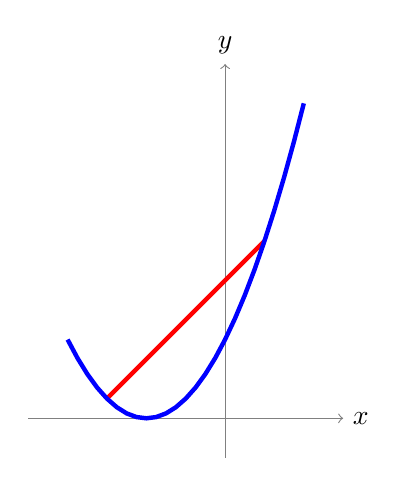
\begin{tikzpicture}
\draw [thin, gray, ->] (0,-0.5) -- (0,4.5)      % draw y-axis line
        node [above, black] {$y$};              % add label for y-axis

    \draw [thin, gray, ->] (-2.5,0) -- (1.5,0)      % draw x-axis line
        node [right, black] {$x$};              % add label for x-axis

    \draw [draw=red,ultra thick] (-1.5,0.25) -- (0.5,2.25);% draw the graph
    \draw[blue, ultra thick, domain=-2:1] plot (\x, {(\x+1)^2});

\end{tikzpicture}
\caption{Esempio funzione convessa: $(x+1)^2$} \label{fig:F1}
\end{figure}

\section{Schemi Iterativi}
Il metodo del gradiente è uno schema iterativo: a partire da un punto iniziale $x^0$, genera una successione di punti $x^1, x^2, ...$ che cerca di migliorare la stima della soluzione, fino al suo raggiungimento. \`E un metodo di tipo iterativo, sfrutta la creazione di una successione $\{x^k\}_{k=0,1,...}$ e, come tutti i metodi di tipo iterativo, deve tener contro di tre aspetti importanti:
\begin{enumerate}
  \item regola per la costruzione delle $x^k$,
  \item convergenza del processo iterativo $\lim_{k \to \infty}x^k = x^*$,
  \item criterio di arresto, infatti il calcolatore non può gestire l'infinito.
\end{enumerate}
Quindi, nel nostro caso (vedi equazione \eqref{min_funz}) dato un punto iniziale $x^0$, per $k=0,1,...$ fino al raggiungimento di un'approssimazione accettabile o a un massimo numero di iterate, calcola il nuovo punto come:
\begin{equation}
    \label{passo_x_k}
    x^{k+1} = x^k + \alpha_k p^k
\end{equation}
dove $\alpha_k > 0$ è la lunghezza del passo (o step length), e $p^k$ è la direzione di ricerca.\\
I metodi di discesa generano una successione $\{f(x^k)\}_k$ monotona decrescente, ossia la successione generata $\{x^k\}_k$ deve essere tale che $f(x^{k+1}) \leqslant f(x^{k})$ per ogni k, e si ha che $f(x^{k+1})=f(x^{k})$ solo se si è arrivati al minimo.
\\
\\
Un vettore $p$ è di discesa per $f$ in $x^k$ se esiste $\overline{\alpha} > 0$ tale che:
\begin{equation}
    \label{vett_discesa}
     f(x^k + \alpha p) < f(x^k ) \quad \alpha \in (0, \overline{\alpha}]
\end{equation}
Per funzioni differenziabili, la condizione per cui $p$ è di discesa in $x^k$ è:
\begin{equation}
    \label{condizione_p_discesa}
     \nabla f(x^k)^T p^k < 0
\end{equation}
Infatti, dallo sviluppo in serie di Tylor:
\begin{equation}
    \label{sviluppo_tylor}
     f(x_0 + \alpha s) = f(x_0) +\alpha\nabla  f(x_0)^T s + \frac{1}{2}\alpha^2 s^T\nabla^2  f(x_0) s + o(\alpha^2)
\end{equation}
sostituendo alla direzione $s$ l'antigradiente in $x^k$ e approssimando ad una funzione lineare nell'intorno di $x^0$, si ottiene:
\begin{equation}
    \label{dimostrazione_discesa}
     f(x^k - \alpha \nabla f(x^k)) = f(x^k) -\alpha\nabla  f(x^k)^T \nabla f(x^k)=f(x^k) -\alpha\|\nabla  f(x^k)\|^2
\end{equation}
dove $\|\nabla  f(x^k)\|^2$ è sempre maggiore di zero, per cui essendoci un meno, sto togliendo a $ f(x^k)$ qualcosa di positivo, quindi ne riduco il valore sempre.
\\
I più significativi metodi di discesa sono i cosiddetti metodi del gradiente, in cui $p^k = -D_k \nabla f(x^k)$, dove $D_k$ è una matrice simmetrica definita positiva di ordine n (si ricorda che una matrice $A$ è definita positiva se $x^T A x > 0 \ \forall x \ne 0$, nella pratica grazie ad un teorema basta verificare la positività di tutti gli autovalori di A per verificare la definita positività).\\
Dalla definita positività di $D_k$ segue che:
\begin{equation}
    \label{discesa_metodo_grad}
     \nabla  f(x^k)^T  p^k = -\nabla f(x^k)^T  D_k \nabla f(x^k) < 0
\end{equation}
se $\nabla f(x^k) \ne 0$, cosicché $p^k$ è sempre direzione di discesa.
In base alla scelta di $D_k$ si definiscono diversi metodi di discesa.


\section{Steepest Descent (SD) o Discesa Ripida}
Si pone $D_k = I_n$, per ogni $k \geqslant 0$. \`E la scelta più semplice, ma spesso implica convergenza lenta. Se considero il punto $x^k$, $f(x^{k+1})$ può essere approssimato come $f(x^k + p) 	\approx f(x^k) + \nabla f(x^k)^T p$, cerco la $p$ che minimizza tale valore. Tra tutti i possibili versori p, quindi con $\| p\| = 1$,  la derivata direzionale $ \nabla f(x^k)^T p$ è minima per $\overline{p} = \frac{-\nabla f(x^k}{\| \nabla f(x^k) \|}$, infatti:
\begin{equation}
    \label{SD1}
     \nabla f(x^k)^T p \geqslant - \| \nabla f(x^k)\| \| p \| \geqslant - \| \nabla f(x^k)\| \ \forall p \ con \ \|p\|=1
\end{equation}
da cui: 
\begin{equation}
    \label{SD2}
     -\| \nabla f(x^k)\| = -\nabla f(x^k)^T \overline{p} = \nabla f(x^k)^T \frac{-\nabla f(x^k}{\| \nabla f(x^k) \|}
\end{equation}
che altro non è che la direzione di più ripida discesa in $x^k$.

\section{Metodo di Newton}
Si pone $D_k = (\nabla^2 f(x^k))^{-1}$, per ogni $k \geqslant 0$, assumendo $\nabla^2 f(x^k)$ definita positiva (ricordando che l'Hessiana definita positiva è condizione sufficiente affinché la funzione sia strettamente positiva).\\
L'idea alla base del metodo di Newton è quella di minimizzare un'approssimazione quadratica $f^k(x)$ di $f(x)$ in $x^k$ (da sviluppo in serie di Tylor):
\begin{equation}
    \label{Newton1}
    \begin{gathered}
     f^k(x) = f(x^k) + \nabla f(x^k)^T (x-x^k) + \frac{1}{2} (x-x^k)^T \nabla^2 f(x^k) (x - x^k)\\
     dove\ x = x^k + h\ da\ cui\ h=x-x^k
    \end{gathered}
\end{equation}
Ponendo a 0 il gradiente di $f^k(x)$, si ottiene:
\begin{equation}
    \label{Newton2}
    \nabla^2f(x^k)^T(x-x^k) + \nabla f(x^k) = 0
\end{equation}
Quindi, risolto il sistema lineare $\nabla^2f(x^k)^Tp = - \nabla f(x^k)$ in cui $p=(x-x^k)$, il punto $x^{k+1}$ risulta:
\begin{equation}
    \label{Newton3}
    x^{k+1} = x^k -\nabla^2f(x^k)^{-1} \nabla f(x^k)
\end{equation}
Questo è il metodo di Newton puro, cioè con $\alpha_k = 1$.

In generale converge molte velocemente in prossimità del minimo, ma spesso il calcolo dell'Hessiana e, a maggior ragione, dell'inversa, risulta impraticabile nei casi reali.

\section{Scelta della Lunghezza del Passo}
In base alla lunghezza del passo $\alpha$, viene assicurata una sufficiente decrescita di $f$ e una velocità di convergenza adeguata. Spesso ci si riferisce alla ricerca della lunghezza del passo con il termine line search.

\subsection{Regola del Passo Costante}
Si tiene fisso il parametro a un valore dato dall'utente. Se il passo è troppo grande si può avere divergenza, se è troppo piccolo convergenza lenta.

\subsection{Regola di Minimizzazione Esatta}
Si cerca il valore di $\alpha_k$ che minimizza $f$ lungo la direzione $p^k$, ossia si risolve un problema di minimo unidimensionale:
\begin{equation}
    \label{min_esatta}
    \underset{\alpha>0}{\min} F(\alpha) = f(x^k + \alpha p^k)
\end{equation}
$\alpha_k$ deve essere tale che annulli la derivata del funzionale $F(\alpha)$:\\ $F'(\alpha) = \nabla f(x^k+\alpha p^k)^T p^k$.\\
Il punto $x^{k+1}$ è il punto in cui il gradiente nel nuovo punto è ortogonale alla direzione di ricerca $p^k$, infatti $\nabla f(x^k+\alpha p^k)^T p^k=0$ per costruzione.\\
Ciò porta a lenta convergenza, poiché ci si sposta sempre di \ang{90} rispetto alla direzione di ricerca precedente, e quindi si ha un andamento verso il minimo che viene detto a zig-zag. 

\subsection{Regola di Minimizzazione Limitata}
Si fissa uno scalare $s>0$ che limita la ricerca di $\alpha_k$:
\begin{equation}
    \label{min_limitata}
    \underset{\alpha \in (0,s]}{\min} F(\alpha) = f(x^k + \alpha p^k)
\end{equation}
\\
Servono algoritmi di ricerca di $\alpha$ sia nel caso esatto che nel caso limitato. Nel caso della ricerca esatta potrebbe essere un'operazione costosa e non necessaria, infatti spesso è meglio cambiare direzione di ricerca piuttosto che trovare la lunghezza migliore per una certa direzione. In tutto ciò però, devo sempre garantire una sufficiente decrescita della mia funzione, ed è qui che la procedura di backtracking viene in aiuto.

\subsection{Backtracking}
Dati $\alpha_0 > 0, c \in (0,1), \rho \in (0,1)$ eseguo la seguente procedura di line search:

\begin{algorithm}
\caption{Line search inesatta}\label{alg:euclid}
\begin{algorithmic}[1]
\Procedure{backtracking}{$\alpha_0, c, \rho$}\Comment{Line search inesatta}
\State $\alpha \gets \alpha_0$
\While{$f(x^k + \alpha p^k) > f(x^k) + c \alpha \nabla f(x^k)^T p^k$}\Comment{Garantisco decrescita}
\State $\alpha \gets \rho\alpha$
\EndWhile
\State $\alpha_k \gets \alpha$
\EndProcedure
\end{algorithmic}
\end{algorithm}
Lo scalare $c$ mi serve a bilanciare il valore del gradiente rispetto a $f$.\\
La condizione di crescita deve soddisfare la regola di Armijo:
\begin{equation}
    \label{armijo1}
    f(x^k + \alpha p^k) \leqslant f(x^k) + c \alpha \nabla f(x^k)^T p^k
\end{equation}
\begin{equation}
    \label{armijo2}
         F( \alpha ) \leqslant I( \alpha ) \equiv F( 0 ) + c \alpha F'(0 )
\end{equation}
\begin{figure}[H]
  	\centering
	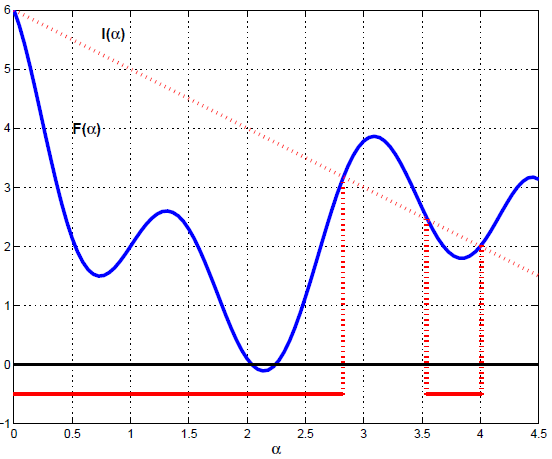
\includegraphics[width=0.5\textwidth]{Immagine_1}
    	\caption{Valori di $\alpha$ che soddisfano la condizione (\ref{armijo2}) in questo esempio particolare}
\end{figure}
$I( \alpha )$ è una retta con pendenza negativa, il suo grafico per piccoli valori di $\alpha$ sta sopra a $F( \alpha )$, quindi la condizione per piccoli valori di $\alpha$ è sicuramente soddisfatta.

\subsection{Barzilai-Borwein}
\`E uno dei metodi più utilizzati per accelerare notevolmente la velocità di convergenza senza dispendio in termini di risorse di calcolo. Si cercano di inglobare informazioni del secondo ordine, quindi relative all'Hessiana, nella scelta della lunghezza del passo $\alpha_k$. In pratica si cercano valori di $\alpha_k$ tali che $\alpha_k \nabla f(x^k) \approx (\nabla^2 f(x^k))^{-1}  \nabla f(x^k)$. Supposto di voler minimizzare una funzione quadratica del tipo $\frac{1}{2} x^T A x$, dove quindi l'Hessiana è $A$, la precedente relazione ci porta ad ottenere:
\begin{equation}
    \label{BB1}
        \frac{1}{\alpha_k} I \approx A	
\end{equation}
per le proprietà di $A$ si ha che:
\begin{equation}
    \label{BB2}
        A (x^{k+1} - x^{k}) = \nabla f(x^{k+1}) -\nabla f( x^{k} )
\end{equation}
eseguendo le seguenti sostituzioni $s^k =(x^{k+1} - x^{k})$ e $y^k=\nabla f(x^{k+1}) -\nabla f( x^{k} )$ che sono la differenza, rispettivamente, di due iterate successive e di due gradienti successivi, posso riscrivere la (\ref{BB2}) come:
\begin{equation}
    \label{BB3}
        A s^k = y^k
\end{equation}
Procedo risolvendo un problema ai minimi quadrati, cioè cerco i valori di $\alpha$ che minimizzano la distanza tra i due termini dell'equazione $\frac{1}{\alpha}  s^k = y^k$:
\begin{equation} 
\label{BB4}
\min_{\alpha} \frac{1}{2} \|\frac{1}{\alpha} s^k - y^k\|^2 
\end{equation}
\begin{equation} 
\label{BB5}
\min_{\alpha} \| s^k -\alpha y^k\|^2 
\end{equation}
Dall'equazione (\ref{BB4}) ricavo $\alpha$ minimo:

\begin{equation} 
\label{BB6}
	\begin{split}
	\min_{\alpha} \frac{1}{2} \|\frac{1}{\alpha} s^k - y^k\|^2& =\\
	 &= \min_{\alpha} \frac{1}{2}\left (\frac{1}{\alpha} s^k - y^k\right)^T\left(\frac{1}{\alpha} s^k - y^k\right)\\
	 &= \min_{\alpha} \frac{1}{2} \left(\left(\frac{1}{\alpha}\right)^2 {s^k}^T s^k + {y^k}^T y^k-2\left(\frac{1}{\alpha}\right){s^k}^T y^k\right)\\
	 & posto\  \frac{1}{\alpha} = \gamma \ ,({y^k}^T y^k)\ non\ dipende\ da\ \alpha,\ lo\ elimino\\
	 &=  \min_{\gamma} \frac{1}{2} \gamma^2 {s^k}^T s^k -\gamma{s^k}^T y^k\\
	 &trovo\ il\ minimo\ ponendo\ la\ derivata\ a\ zero\\
	 &\Rightarrow \gamma {s^k}^T s^k -{s^k}^T y^k = 0\\
	 & \gamma = \frac{{s^k}^T y^k}{{s^k}^T s^k}, \ da\ cui\\
	 & \alpha^{BB1} = \frac{{s^k}^T s^k}{{s^k}^T y^k}\\
	 & e\ in\ modo\ analogo\ trovo \\
	 & \alpha^{BB2} = \frac{{s^k}^T y^k}{{y^k}^T y^k}
	\end{split}
\end{equation}
Queste regole, prescindendo dalla conoscenza di A, possono essere inglobate a costo zero in un algoritmo per problemi non lineari (con line search inesatta) anche con vincoli semplici per cui l'Hessiana è difficilmente calcolabile.\\
Si osserva che $\alpha^{BB2} \leqslant \alpha^{BB1}$. Spesso si utilizzano tecniche di alternanza, per cui si eseguono alcune iterazioni con il primo parametro, altre iterazioni con il secondo parametro e così via.

\section{Risultati di Convergenza}
Andiamo ora a ragionare sui risultati ottenuti attraverso l'utilizzo dei metodi del gradiente nel nostro caso. Infatti, la successione generata dai metodo del gradiente può non avere punti di accumulazione: se la funzione $f$ non ha minimi locali, la successione $\{x^k\}$ può non essere limitata. Se però sappiamo che l'insieme di livello $\mathcal{L}_{\leqslant f(x^0)}(f) = \{x: f(x) \leqslant f(x^0)\}$ è limitato, e la scelta della lunghezza del passo forza la decrescita della funzione, allora la successione $\{x^k\}$ è limitata e dunque ha almeno un punto di accumulazione, ma non sappiamo ancora se corrisponde ad un minimo e se è unico.\\

Dalla sviluppo in serie di Tylor del primo ordine di f in $x^k$ noto che la condizione che crea problemi quando ci si avvicina ad un punto stazionario (cioè con gradiente nullo) è la seguente:
\begin{equation} 
\label{coseno_nullo}
	\cos (\theta_k) = \frac{\nabla f(x^k)^T p^k}{\| \nabla f(x^k)\| \|p^k\|} \rightarrow 0 
\end{equation}
in tal caso la funzione non presenta sufficiente decrescita e il metodo resta incollato al punto di non stazionarietà.

\subsection{Direzioni Gradient Related}
Una successione di direzioni $\{p^k\}$ si dice gradient related a $\{x^k\}$ se per ogni sotto-successione $\{x^j\}_{j \in J}$ convergente ad un punto di non stazionarietà, la corrispondente sotto-successione $\{p^j\}_{j \in J}$  è limitata e soddisfa la condizione:
\begin{equation} 
\label{grad_rel}
	\lim_{j \rightarrow \infty} \sup_{j \in J} {\nabla f(x^j)^T p^j} < 0
\end{equation}
Se dunque $p^k$ è gradient related, segue che se una sotto-successione $\{\nabla f(x^j)\}_{j \in J}$ tende a un vettore non nullo, la corrispondente sotto-successione$\{p^j\}_{j \in J}$ è limitata e non può tendere a essere ortogonale al gradiente, ossia  $p^k$ non diventa né troppo piccola, né troppo grande e l'angolo tra $p^k$ e $\nabla f(x^k)$ non si avvicina a $\frac{\pi}{2}$.\\

Il presupposto per avere direzioni gradient related è quella di porre condizioni a priori su $p^k$ che generalmente sono soddisfatte e non impongono grosse restrizioni. Nel caso dei metodi del gradiente, per cui $p^k = -D_k \nabla f(x^k)$, una condizione è quella di imporre gli autovalori della matrice simmetrica $D_k$ definita positiva limitati dal basso e dall'alto da costanti positive indipendenti da $k$:
\begin{equation} 
\label{condiz_autoval1}
	\exists \lambda_1,\lambda_2\quad  \lambda_1 \| z \|^2 \leqslant z^T D_k z \leqslant  \lambda_2 \| z \|^2 ,\ \forall z \in R^n,\ k=0,1,...
\end{equation}
Di conseguenza:
\begin{multline}
	| \nabla f(x^k)^T p^k|= | \nabla f(x^k)^T D_k \nabla f(x^k)| \geqslant  \lambda_1 \| \nabla f(x^k) \|^2 \\
	\| p^k \|^2 = | \nabla f(x^k)^T {D_k}^2 \nabla f(x^k)| \leqslant \lambda_2 \| \nabla f(x^k) \|^2
\end{multline}
Pertanto, finché $\nabla f(x^k)$ non tende a zero, $\nabla f(x^k)$ e $p^k$ non possono diventare asintoticamente ortogonali e quindi il coseno non diventa mai nullo.\\

Un altro risultato utile a garantire la convergenza del metodo nel nostro caso è dato dal seguente teorema.\\
Sia $f$ di classe $\mathcal{C}^1$ in $\mathcal{L}_{\leqslant f(x^0)}(f)$, sia $\{ x^k\}$ una successione generata da un metodo del gradiente con $\{ p^k\}$ gradient related e $\alpha_k$ scelta con una regola qualsiasi (minimizzazione esatta, limitata o backtracking). Allora ogni punto limite di $\{ x^k\}$ è punto di stazionarietà di $f$.

\subsection{Teorema della Cattura}
Sia $f$ di classe $\mathcal{C}^1$ in $L_{\leqslant f(x^0)}(f)$, sia $\{ x^k\}$ una successione tale che $\{ f(x^k)\}$ sia monotona non crescente ed è generata da un metodo del gradiente per cui ogni punto  di accumulazione è punto di stazionarietà di $f$.\\
Siano $\overline{\alpha} > 0, L > 0 $ tali che $\alpha_k \leqslant \overline{\alpha}$ e $\alpha_k \leqslant \overline{\alpha}$.\\
Sia $x^*$ l'unico punto di minimo locale di $f$ in un aperto.\\
Allora esiste un aperto S contenente $x^*$ tale che se $x^{\overline{k}} \in S$ per un qualche $\overline{k} > 0$, allora $x^k \in S$ per ogni $k \geqslant \overline{k}$ e $x^k \rightarrow x^*$ per $k \rightarrow +\infty$.

\section{Velocità di Convergenza}
Dopo aver studiato i teoremi che garantiscono la convergenza dei metodi del gradienti nel nostro caso, passiamo a verificare come analizzarne la velocità di convergenza.\\

Si assuma che $\{x^k\}$ sia una successione convergente a un punto stazionario $x^*$. La velocità di convergenza viene studiata asintoticamente, usando una funzione errore $e : R^n \rightarrow R$, tale che $e(x) \geqslant 0$ per ogni $x \in R^n$ e $e(x^*) = 0$. Un esempio di funzioni di errore sono le seguenti:
\begin{equation}
\label{funz_errore1}
	e(x) = \| x - x^*\|
\end{equation}
\begin{equation}
\label{funz_errore2}
	e(x) = \| f(x) - f(x^*)\|
\end{equation}
Lo studio asintotico viene condotto confrontando $\{e(x^k )\}$ con qualche successione standard. Si dice che:

$\rightarrow$ la convergenza è lineare o geometrica se $\exists q > 0$ e $\beta \in (0,1)$ tali che
\begin{equation}
	e(x^k) \leqslant q \beta^k \quad k \geqslant 0
\end{equation}

$\quad$La convergenza lineare è garantita se:
\begin{equation}
	\lim_{k \rightarrow \infty} \sup \frac{e(x^{k+1})}{e(x^k)} \leqslant \beta \quad \beta \in (0,1)
\end{equation}
\\

$\rightarrow$ la convergenza è super-lineare se $\forall \beta \in (0,1)$ e $\exists q > 0$ tali che
\begin{equation}
	e(x^k) \leqslant q \beta^k \quad k \geqslant 0
\end{equation}

$\quad$La convergenza super-lineare è garantita se:
\begin{equation}
	\lim_{k \rightarrow \infty} \sup \frac{e(x^{k+1})}{e(x^k)} = 0
\end{equation}
\\

La convergenza super-lineare può essere quantificata confrontando $\{e(x^k )\}$ con la successione${(\beta^t)}^k$ , $t \geqslant 1, k \geqslant 0$; si dice che $\{e(x^k )\}$ converge super-linearmente con ordine almeno $t$ se esiste $q > 0,\ \beta \in (0, 1),\ t > 1$ per cui:
\begin{equation}
	e(x^k) \leqslant q {(\beta^t)}^k \quad k \geqslant 0
\end{equation}
per $t = 2$ si parla di velocità di convergenza quadratica. La convergenza super-lineare di ordine t è garantita se:
\begin{equation}
	\lim_{k \rightarrow \infty} \sup \frac{e(x^{k+1})}{e(x^k)^t} < \infty
\end{equation}
\\
Un altro risultato interessante è dato dal seguente teorema.\\
Sia $f(x) = \frac{1}{2} x^T A x$, $A$ simmetrica definita positiva. Sia $\{x^k\}$ generata dal metodo Steepest Descent, dove quindi $x^{k+1} = x^k - \alpha_k \nabla f(x^k)$, $\alpha_k$ è scelta con la regola di minimizzazione esatta.\\
Allora per ogni $k$ si ha:
\begin{equation}
	f(x^{k+1}) \leqslant \left(\frac{M - m}{M + m}\right)^2 f (x^k)
\end{equation}
dove M e m sono, rispettivamente, il più grande e il più piccolo autovalore di A.\\
Poiché A è definita positiva, ho il minimo in $x = 0$. Se $M \approx m$, ho forte smorzamento da un'iterazione all'altra, arrivando in fretta al minimo, infatti più M e m sono simili, più le curve di livello sono circonferenze. Nel caso opposto, quindi dove $M \gg m$, ho curve di livello molto ellittiche e quindi un andamento a zig zag e una lenta convergenza.\\
Stesso risultato più generale si ha con $f : R^n \rightarrow R$, $f \in \mathcal{C}^2$. Considerata la sequenza generata del metodo di discesa ripida combinata con una procedura di backtracking, se si assume che $\{ x^k\}$ converga ad un punto di minimo locale forte $x^*$ in cui l'Hessiana è definita positiva, allora
\begin{equation}
	f(x^{k+1}) - f(x^*) \leqslant \left(\frac{k\left(\nabla^2  f(x^*)\right) - 1}{k\left(\nabla^2  f(x^*)\right) + 1}\right)^2 \left(f(x^k) - f(x^*)\right)
\end{equation}
dove $k(A) = \frac{M}{m} \Rightarrow \left(\frac{M- m}{M+m}\right)^2 = \left(\frac{\frac{M}{m}- 1 }{\frac{M}{m} + 1 }\right)^2 = \left(\frac{k(A)- 1}{k(A)+1}\right)^2 $

 
\end{document}